\section{Exercises}

%________________
\subsection{Introduction to multiple regression}

% 1

\eoce{\qt{Baby weights, Part I} \label{babiesWeight} The Child Health and Development Studies investigate a range of topics. One study considered all pregnancies between 1960 and 1967 among women in the Kaiser Foundation Health Plan in the San Francisco East Bay area. Here, we study the relationship between smoking and weight of the baby. The variable \texttt{smoke} is coded 1 if the mother is a smoker, and 0 if not. The summary table below shows the results of a linear regression model for predicting the average birth weight of babies, measured in ounces, based on the smoking status of the mother. \footfullcite{data:babies}
\begin{center}
\begin{tabular}{rrrrr}
  \hline
 & Estimate & Std. Error & t value & Pr($>$$|$t$|$) \\ 
  \hline
(Intercept) & 123.05 & 0.65 & 189.60 & 0.0000 \\ 
  smoke & -8.94 & 1.03 & -8.65 & 0.0000 \\ 
   \hline
\end{tabular}
\end{center}
The variability within the smokers and non-smokers are about equal and the distributions are symmetric. With these conditions satisfied, it is reasonable to apply the model. (Note that we don't need to check linearity since the predictor has only two levels.)
\begin{parts}
\item Write the equation of the regression line.
\item Interpret the slope in this context, and calculate the predicted birth weight of babies born to smoker and non-smoker mothers.
\item Is there a statistically significant relationship between the average birth weight and smoking?
\end{parts}
}{}

% 2

\eoce{\qt{Baby weights, Part II} \label{babiesParity} Exercise~\ref{babiesWeight} introduces a data set on birth weight of babies. Another variable we consider is \texttt{parity}, which is 0 if the child is the first born, and 1 otherwise. The summary table below shows the results of a linear regression model for predicting the average birth weight of babies, measured in ounces, from \texttt{parity}. 
\begin{center}
\begin{tabular}{rrrrr}
  \hline
 & Estimate & Std. Error & t value & Pr($>$$|$t$|$) \\ 
  \hline
(Intercept) & 120.07 & 0.60 & 199.94 & 0.0000 \\ 
  parity & -1.93 & 1.19 & -1.62 & 0.1052 \\ 
   \hline
\end{tabular}
\end{center}
\begin{parts}
\item Write the equation of the regression line.
\item Interpret the slope in this context, and calculate the predicted birth weight of first borns and others.
\item Is there a statistically significant relationship between the average birth weight and parity?
\end{parts}
}{}

\textB{\newpage}

% 3

\eoce{\qt{Baby weights, Part III\label{babiesMR}} We considered the variables \texttt{smoke} and \texttt{parity}, one at a time, in modeling birth weights of babies in Exercises~\ref{babiesWeight} and \ref{babiesParity}. A more realistic approach to modeling infant weights is to consider all possibly related variables at once. Other variables of interest include length of pregnancy in days (\texttt{gestation}), mother's age in years (\texttt{age}), mother's height in inches (\texttt{height}), and mother's pregnancy weight in pounds (\texttt{weight}). Below are three observations from this data set. 
\begin{center}
\begin{tabular}{r c c c c c c c}
  \hline
 & bwt & gestation & parity & age & height & weight & smoke \\ 
  \hline
1 & 120 & 284 &   0 &  27 &  62 & 100 &   0 \\ 
  2 & 113 & 282 &   0 &  33 &  64 & 135 &   0 \\ 
$\vdots$ & $\vdots$ & $\vdots$ &   $\vdots$ &  $\vdots$ &  $\vdots$ & $\vdots$ &   $\vdots$ \\ 
  1236 & 117 & 297 &   0 &  38 &  65 & 129 &   0 \\ 
   \hline
\end{tabular}
\end{center}
The summary table below shows the results of a regression model for predicting the average birth weight of babies based on all of the variables included in the data set.
\begin{center}
\begin{tabular}{rrrrr}
  \hline
 & Estimate & Std. Error & t value & Pr($>$$|$t$|$) \\ 
  \hline
(Intercept) & -80.41 & 14.35 & -5.60 & 0.0000 \\ 
  gestation & 0.44 & 0.03 & 15.26 & 0.0000 \\ 
  parity & -3.33 & 1.13 & -2.95 & 0.0033 \\ 
  age & -0.01 & 0.09 & -0.10 & 0.9170 \\ 
  height & 1.15 & 0.21 & 5.63 & 0.0000 \\ 
  weight & 0.05 & 0.03 & 1.99 & 0.0471 \\ 
  smoke & -8.40 & 0.95 & -8.81 & 0.0000 \\ 
   \hline
\end{tabular}
\end{center}
\begin{parts}
\item Write the equation of the regression line that includes all of the variables.
\item Interpret the slopes of \texttt{gestation} and \texttt{age} in this context.
\item The coefficient for \texttt{parity} is different than in the linear model shown in Exercise~\ref{babiesParity}. Why might there be a difference?
\item Calculate the residual for the first observation in the data set.
\item The variance of the residuals is 249.28, and the variance of the birth weights of all babies in the data set is 332.57. Calculate the $R^2$ and the adjusted $R^2$. Note that there are 1,236 observations in the data set.
\end{parts}
}{}

\textB{\newpage}

% 4

\eoce{\qt{Absenteeism} \label{daysAbsent} Researchers interested in the relationship between absenteeism from school and certain demographic characteristics of children collected data from 146 randomly sampled students in rural New South Wales, Australia, in a particular school year. Below are three observations from this data set. 
\begin{center}
\begin{tabular}{r c c c c}
\hline
 	& eth 	& sex 	& lrn 		& days \\   
\hline
1 	& 0 		& 1 		& 1 		&   2 \\ 
2 	& 0 		& 1 		& 1 		&  11 \\ 
$\vdots$ & $\vdots$ & $\vdots$ &   $\vdots$ &  $\vdots$  \\ 
146 & 1 		& 0 		& 0 		&  37 \\ 
   \hline
\end{tabular}
\end{center}
The summary table below shows the results of a linear regression model for predicting the average number of days absent based on ethnic background (\texttt{eth}: 0 - aboriginal, 1 - not aboriginal), sex (\texttt{sex}: 0 - female, 1 - male), and learner status (\texttt{lrn}: 0 - average learner, 1 - slow learner). \footfullcite{data:quine}
\begin{center}
\begin{tabular}{rrrrr}
  \hline
 & Estimate & Std. Error & t value & Pr($>$$|$t$|$) \\ 
  \hline
(Intercept) & 18.93 & 2.57 & 7.37 & 0.0000 \\ 
  eth & -9.11 & 2.60 & -3.51 & 0.0000 \\ 
  sex & 3.10 & 2.64 & 1.18 & 0.2411 \\ 
  lrn & 2.15 & 2.65 & 0.81 & 0.4177 \\ 
   \hline
\end{tabular}
\end{center}
\begin{parts}
\item Write the equation of the regression line.
\item Interpret each one of the slopes in this context.
\item Calculate the residual for the first observation in the data set: a student who is aboriginal, male, a slow learner, and missed 2 days of school.
\item The variance of the residuals is 240.57, and the variance of the number of absent days for all students in the data set is 264.17. Calculate the $R^2$ and the adjusted $R^2$. Note that there are 146 observations in the data set.
\end{parts}
}{}

% 5

\eoce{\qt{GPA} \label{gpa} A survey of 55 Duke University students asked about their GPA, number of hours they study at night, number of nights they go out, and their gender. Summary output of the regression model is shown below. Note that male is coded as 1. 
\begin{center}
\begin{tabular}{rrrrr}
  \hline
 & Estimate & Std. Error & t value & Pr($>$$|$t$|$) \\ 
  \hline
(Intercept) & 3.45 & 0.35 & 9.85 & 0.00 \\ 
  studyweek & 0.00 & 0.00 & 0.27 & 0.79 \\ 
  sleepnight & 0.01 & 0.05 & 0.11 & 0.91 \\ 
  outnight & 0.05 & 0.05 & 1.01 & 0.32 \\ 
  gender & -0.08 & 0.12 & -0.68 & 0.50 \\ 
   \hline
\end{tabular}
\end{center}
\begin{parts}
\item Calculate a 95\% confidence interval for the coefficient of gender in the model, and interpret it in the context of the data.
\item Would you expect a 95\% confidence interval for the slope of the remaining variables to include 0? Explain
\end{parts}
}{}

\textB{\newpage}

% 6

\eoce{\qt{Cherry trees} Timber yield is approximately equal to the volume of a tree, however, this value is difficult to measure without first cutting the tree down. Instead, other variables, such as height and diameter, may be used to predict a tree's volume and yield. Researchers wanting to understand the relationship between these variables for black cherry trees collected data from 31 such trees in the Allegheny National Forest, Pennsylvania. Height is measured in feet, diameter in inches (at 54 inches above ground), and volume in cubic feet.\footfullcite{Hand:1994}
\begin{table}[ht]
\begin{center}
\begin{tabular}{rrrrr}
  \hline
 & Estimate & Std. Error & t value & Pr($>$$|$t$|$) \\ 
  \hline
(Intercept) & -57.99 & 8.64 & -6.71 & 0.00 \\ 
height & 0.34 & 0.13 & 2.61 & 0.01 \\ 
diameter & 4.71 & 0.26 & 17.82 & 0.00 \\ 
   \hline
\end{tabular}
\end{center}
\end{table}
\begin{parts}
\item Calculate a 95\% confidence interval for the coefficient of height, and interpret it in the context of the data.
\item One tree in this sample is 79 feet tall, has a diameter of 11.3 inches, and is 24.2 cubic feet in volume. Determine if the model overestimates or underestimates the volume of this tree, and by how much.
\end{parts}
}{}


%________________
\subsection{Model selection}

% 7

\eoce{\qt{Baby weights, Part IV} \label{babiesMRfinal} Exercise~\ref{babiesMR} considers a model that predicts a newborn's weight using several predictors. Use the regression table below, which summarizes the model, to answer the following questions. If necessary, refer back to Exercise~\ref{babiesMR} for a reminder about the meaning of each variable.
\begin{center}
\begin{tabular}{rrrrr}
  \hline
 & Estimate & Std. Error & t value & Pr($>$$|$t$|$) \\ 
  \hline
(Intercept) & -80.41 & 14.35 & -5.60 & 0.0000 \\ 
  gestation & 0.44 & 0.03 & 15.26 & 0.0000 \\ 
  parity & -3.33 & 1.13 & -2.95 & 0.0033 \\ 
  age & -0.01 & 0.09 & -0.10 & 0.9170 \\ 
  height & 1.15 & 0.21 & 5.63 & 0.0000 \\ 
  weight & 0.05 & 0.03 & 1.99 & 0.0471 \\ 
  smoke & -8.40 & 0.95 & -8.81 & 0.0000 \\ 
   \hline
\end{tabular}
\end{center}
\begin{parts}
\item Determine which variables, if any, do not have a significant linear relationship with the outcome and should be candidates for removal from the model. If there is more than one such variable, indicate which one should be removed first.
\item The summary table below shows the results of the model with the \var{age} variable removed. Determine if any other variable(s) should be removed from the model.
\begin{center}
\begin{tabular}{rrrrr}
  \hline
 & Estimate & Std. Error & t value & Pr($>$$|$t$|$) \\ 
  \hline
(Intercept) & -80.64 & 14.04 & -5.74 & 0.0000 \\ 
  gestation & 0.44 & 0.03 & 15.28 & 0.0000 \\ 
  parity & -3.29 & 1.06 & -3.10 & 0.0020 \\ 
  height & 1.15 & 0.20 & 5.64 & 0.0000 \\ 
  weight & 0.05 & 0.03 & 2.00 & 0.0459 \\ 
  smoke & -8.38 & 0.95 & -8.82 & 0.0000 \\ 
   \hline
\end{tabular}
\end{center}
\end{parts}
}{}

\textB{\newpage}

% 8

\eoce{\qt{Absenteeism, Part II} Exercise~\ref{daysAbsent} considers a model that predicts the number of days absent using three predictors: ethnic background (\var{eth}), gender (\var{sex}), and learner status (\var{lrn}). Use the regression table below to answer the following questions. If necessary, refer back to Exercise~\ref{daysAbsent} for additional details about each variable. 
\begin{center}
\begin{tabular}{rrrrr}
  \hline
 & Estimate & Std. Error & t value & Pr($>$$|$t$|$) \\ 
  \hline
(Intercept) & 18.93 & 2.57 & 7.37 & 0.0000 \\ 
  eth & -9.11 & 2.60 & -3.51 & 0.0000 \\ 
  sex & 3.10 & 2.64 & 1.18 & 0.2411 \\ 
  lrn & 2.15 & 2.65 & 0.81 & 0.4177 \\ 
   \hline
\end{tabular}
\end{center}
 \begin{parts}
\item Determine which variables, if any, do not have a significant linear relationship with the outcome and should be candidates for removal from the model. If there is more than one such variable, indicate which one should be removed first.
\item The summary table below shows the results of the regression we refit after removing learner status from the model. Determine if any other variable(s) should be removed from the model.
\begin{center}
\begin{tabular}{rrrrr}
  \hline
 & Estimate & Std. Error & t value & Pr($>$$|$t$|$) \\ 
  \hline
(Intercept) & 19.98 & 2.22 & 9.01 & 0.0000 \\ 
  eth & -9.06 & 2.60 & -3.49 & 0.0006 \\ 
  sex & 2.78 & 2.60 & 1.07 & 0.2878 \\ 
   \hline
\end{tabular}
\end{center}
\end{parts}
}{}

% 9

\eoce{\qt{Baby weights, Part V} Exercise~\ref{babiesMR} provides regression output for the full model (including all explanatory variables available in the data set) for predicting birth weight of babies. In this exercise we consider a forward-selection algorithm and add variables to the model one-at-a-time. The table below shows the p-value and adjusted $R^2$ of each model where we include only the corresponding predictor. Based on this table, which variable should be added to the model first?\vspace{0.5mm}
\begin{center}
\begin{tabular}{l c c c c c c}
\hline
variable		& gestation			& parity	& age	& height 				& weight 				& smoke \\
\hline
p-value		& $2.2 \times 10^{-16}$	& 0.1052	& 0.2375	& $2.97 \times 10^{-12}$	& $8.2 \times 10^{-8}$	& $2.2 \times 10^{-16}$ \\
$R_{adj}^2$	& 0.1657				& 0.0013	& 0.0003	& 0.0386				& 0.0229				& 0.0569 \\
\hline
\end{tabular}
\end{center}
}{}


% 10

\eoce{\qt{Absenteeism, Part III} Exercise~\ref{daysAbsent} provides regression output for the full model, including all explanatory variables available in the data set, for predicting the number of days absent from school. In this exercise we consider a forward-selection algorithm and add variables to the model one-at-a-time. The table below shows the p-value and adjusted $R^2$ of each model where we include only the corresponding predictor. Based on this table, which variable should be added to the model first?\vspace{0.5mm}
\begin{center}
\begin{tabular}{l c c c}
\hline
variable		& ethnicity		& sex	& learner status	 \\
\hline
p-value		& 0.0007		& 0.3142	& 0.5870	 \\
$R_{adj}^2$	& 0.0714		& 0.0001	& 0 \\
\hline
\end{tabular}
\end{center}
}{}


\textB{\newpage}

%________________
\subsection{Checking model assumptions using graphs}


% 11

\eoce{\qt{Baby weights, Part V} Exercise~\ref{babiesMRfinal} presents a regression model for predicting the average birth weight of babies based on length of gestation, parity, height, weight, and smoking status of the mother. Determine if the model assumptions are met using the plots below. If not, describe how to proceed with the analysis.
\begin{center}
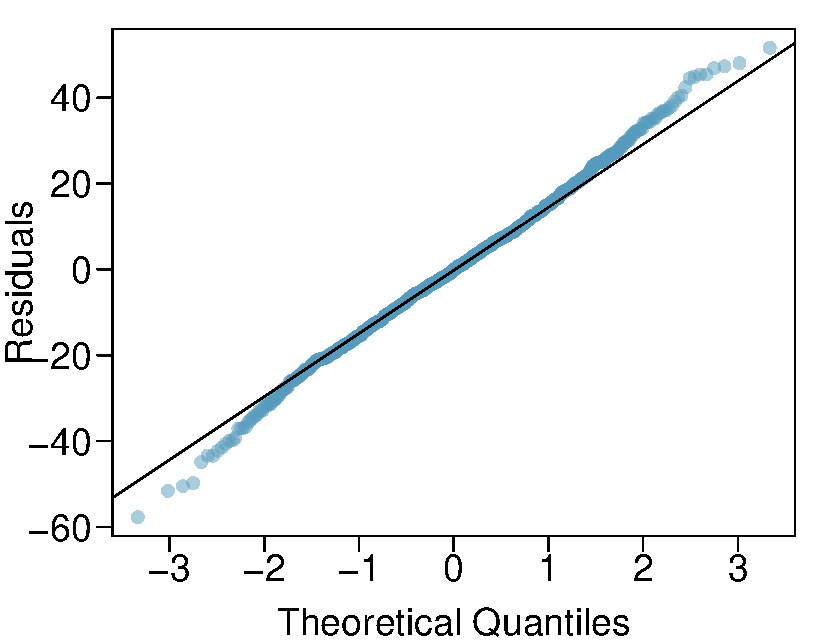
\includegraphics[width=0.4\textwidth]{ch_regr_mult_and_log/figures/eoce/babies/lmBabies2normProbRes} \hspace{5mm}
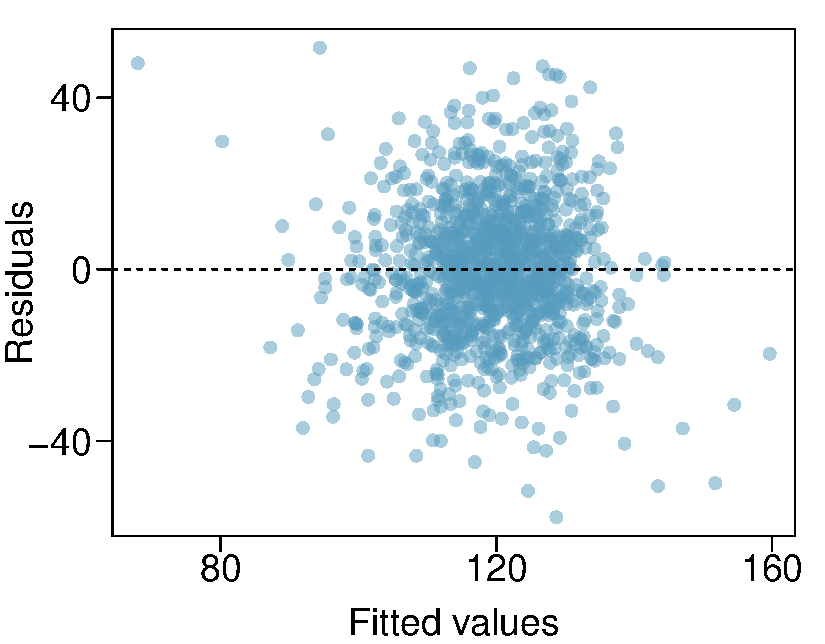
\includegraphics[width=0.4\textwidth]{ch_regr_mult_and_log/figures/eoce/babies/lmBabies2ResFit}\\[3mm]
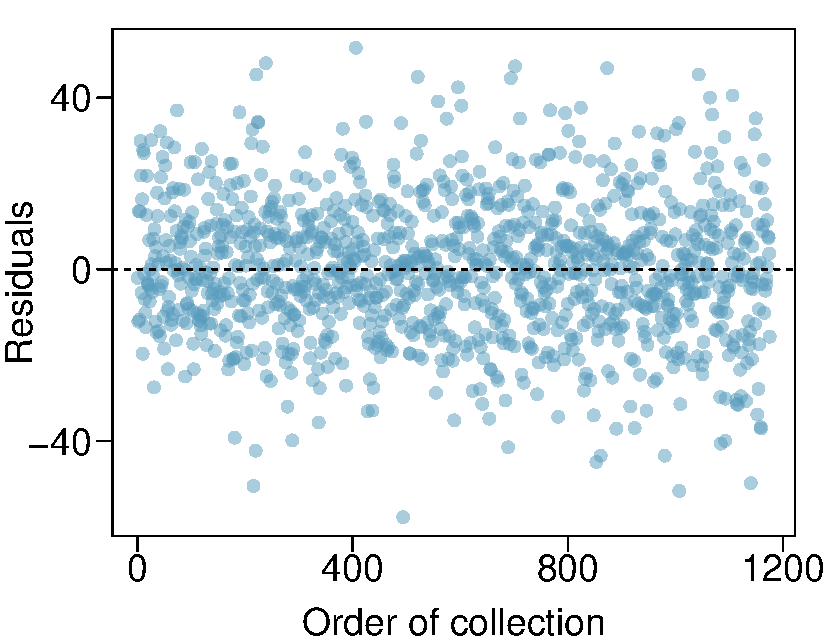
\includegraphics[width=0.4\textwidth]{ch_regr_mult_and_log/figures/eoce/babies/lmBabies2resOrder} \hspace{5mm}
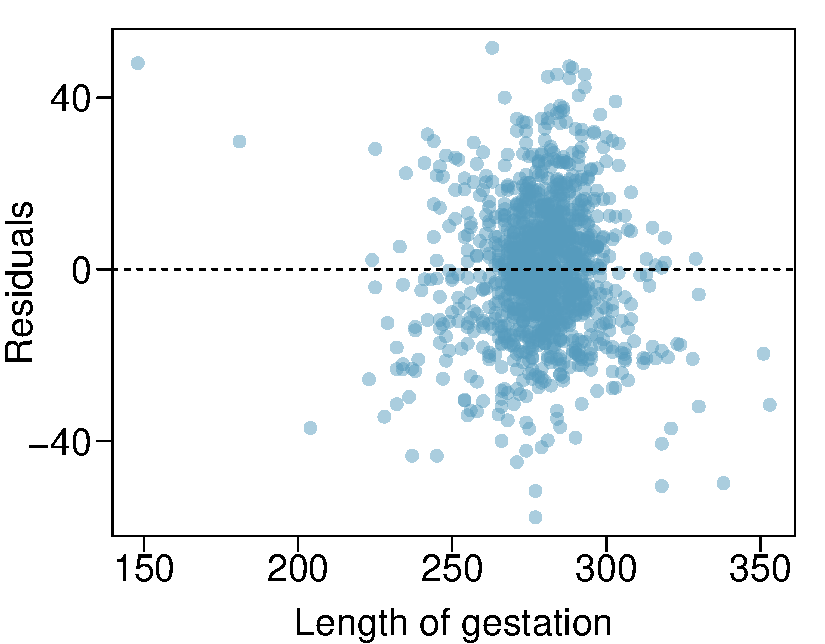
\includegraphics[width=0.4\textwidth]{ch_regr_mult_and_log/figures/eoce/babies/lmBabies2resGest}\\[3mm]  
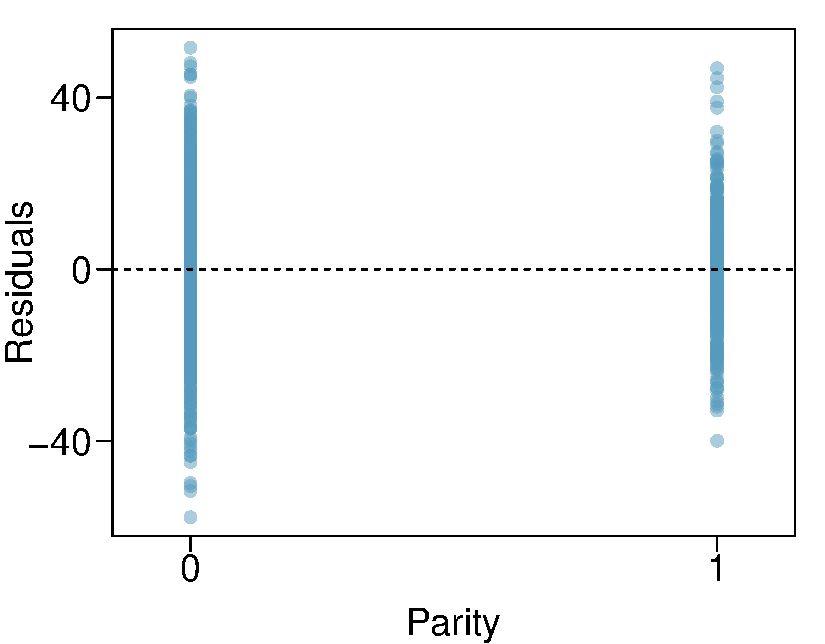
\includegraphics[width=0.4\textwidth]{ch_regr_mult_and_log/figures/eoce/babies/lmBabies2resParity} \hspace{5mm}
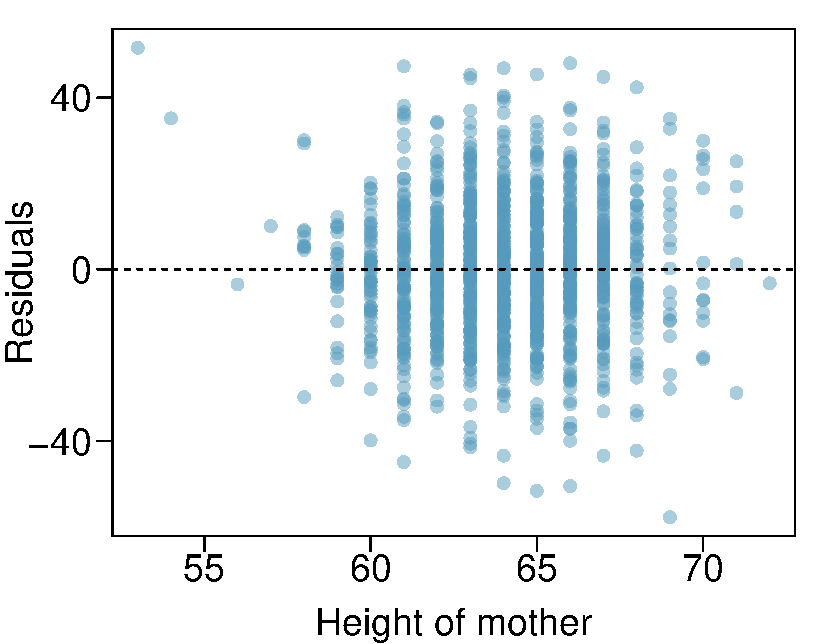
\includegraphics[width=0.4\textwidth]{ch_regr_mult_and_log/figures/eoce/babies/lmBabies2resHgt}\\[3mm]
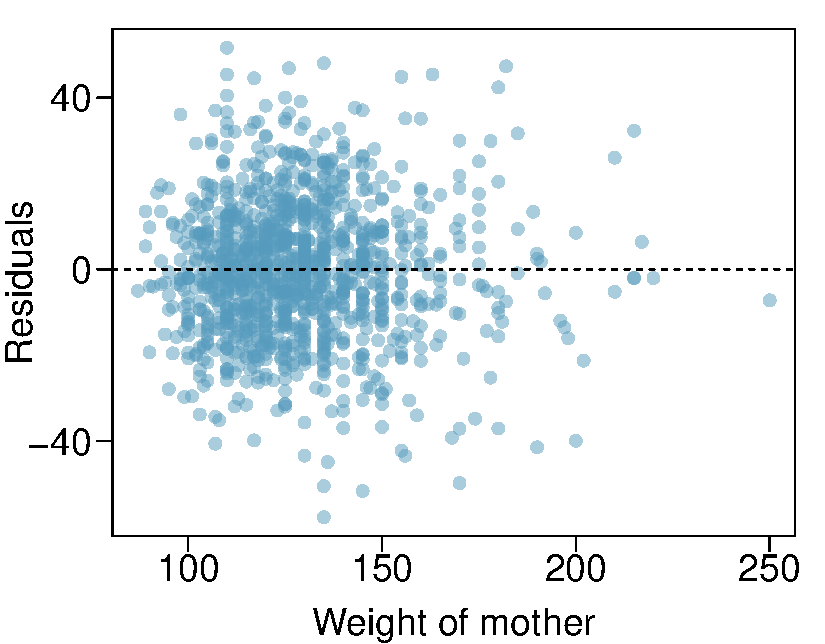
\includegraphics[width=0.4\textwidth]{ch_regr_mult_and_log/figures/eoce/babies/lmBabies2resWgt} \hspace{5mm}
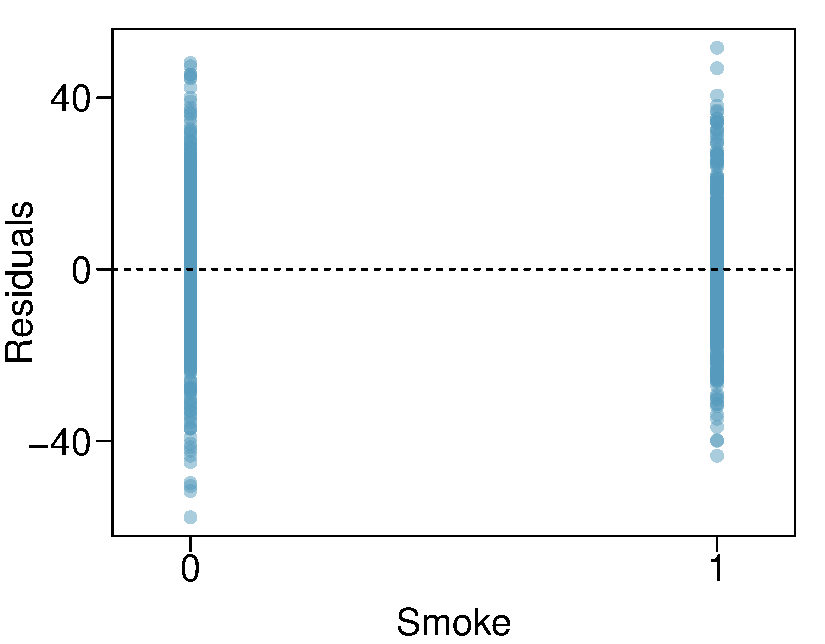
\includegraphics[width=0.4\textwidth]{ch_regr_mult_and_log/figures/eoce/babies/lmBabies2resSmoke} 
\end{center}
}{}

% 12

\eoce{\qt{GPA and IQ} A regression model for predicting GPA from gender and IQ was fit, and both predictors were found to be statistically significant. Using the plots given below, determine if this regression model is appropriate for these data.
\begin{center}
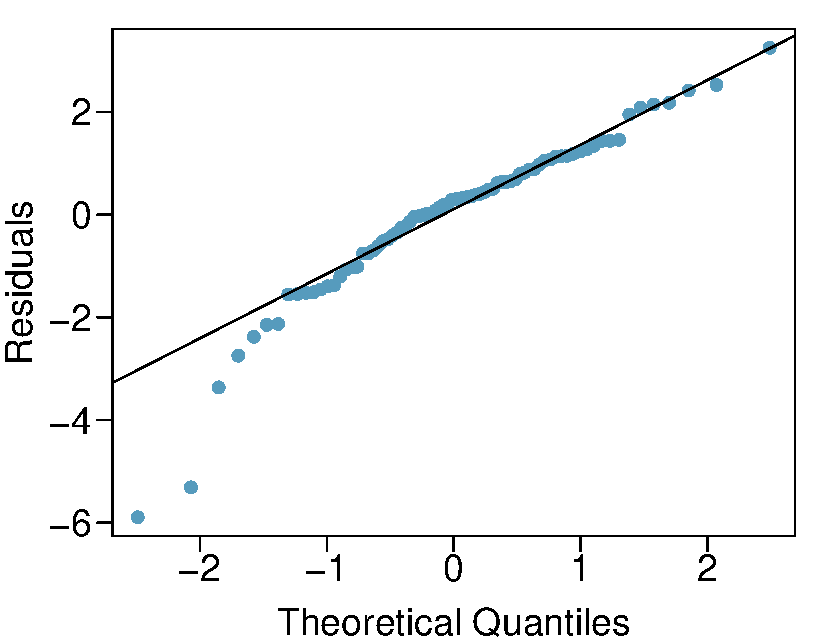
\includegraphics[width=0.47\textwidth]{ch_regr_mult_and_log/figures/eoce/education/lmEduNormProbRes}\hspace{3mm}
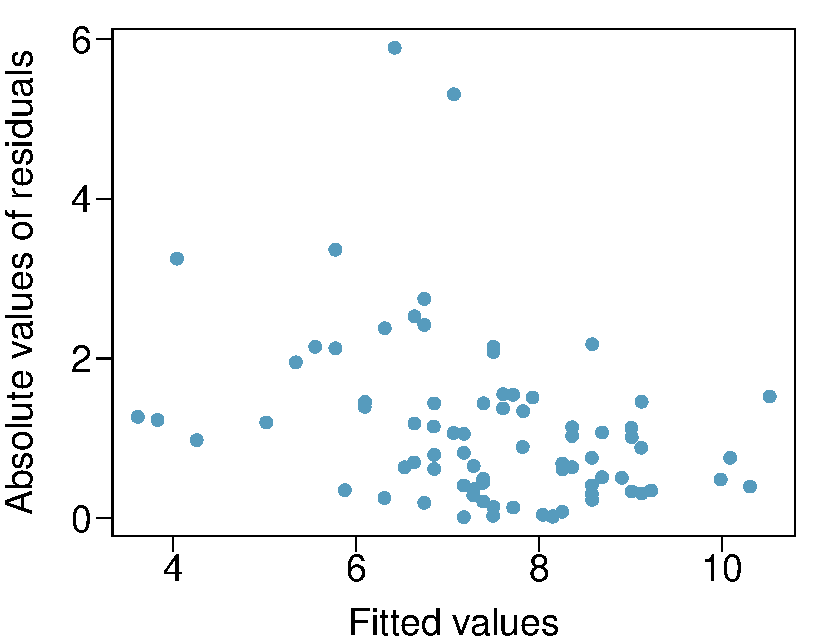
\includegraphics[width=0.47\textwidth]{ch_regr_mult_and_log/figures/eoce/education/lmEduAbsResFit}\\[5mm]
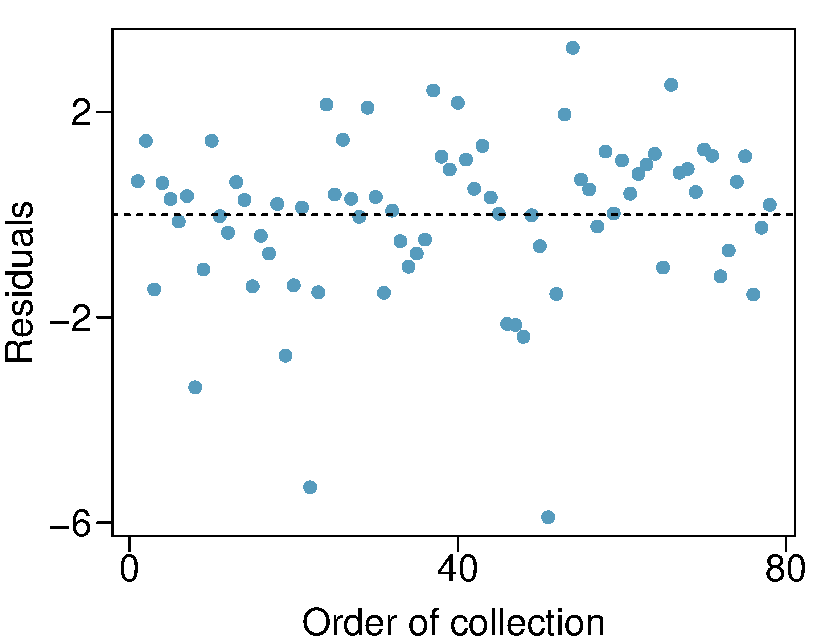
\includegraphics[width=0.47\textwidth]{ch_regr_mult_and_log/figures/eoce/education/lmEduResOrder}\hspace{3mm}
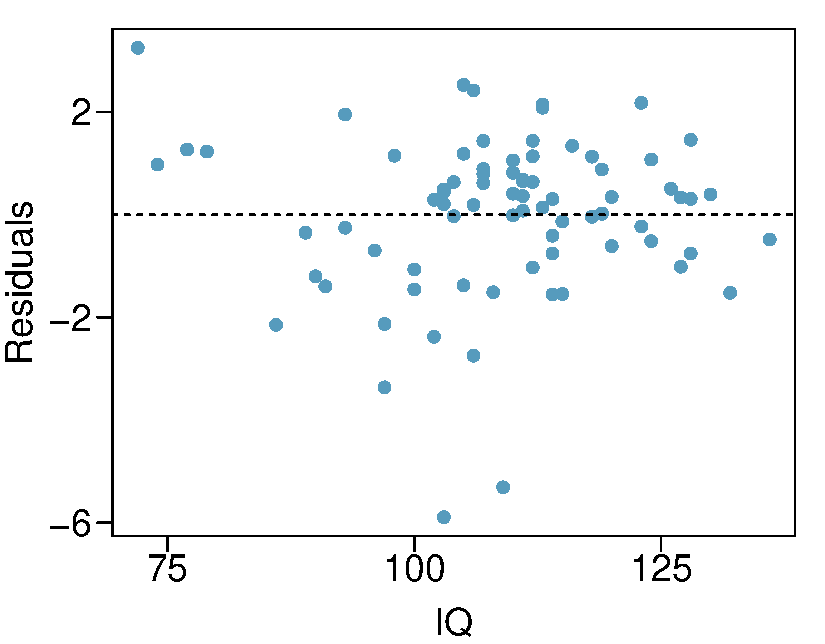
\includegraphics[width=0.47\textwidth]{ch_regr_mult_and_log/figures/eoce/education/lmEduResIQ}\\[5mm]
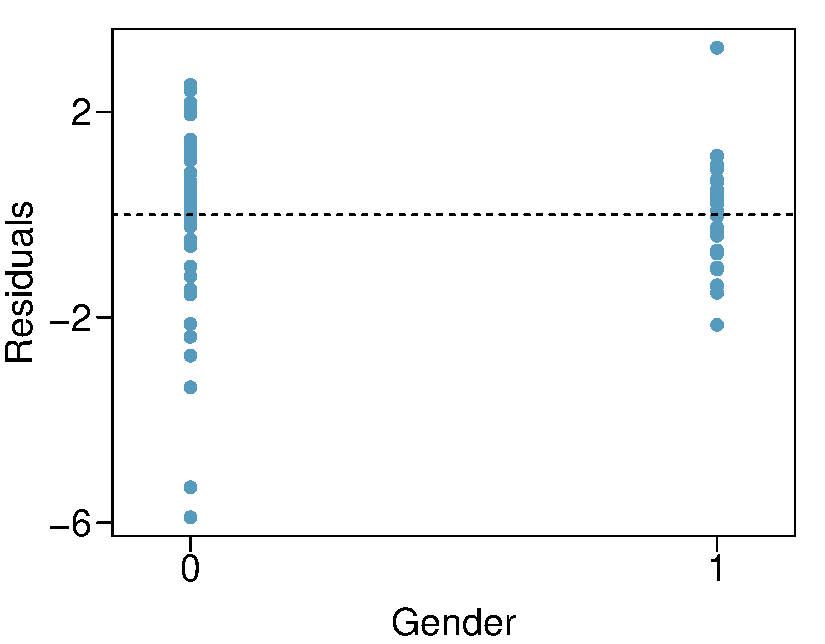
\includegraphics[width=0.5\textwidth]{ch_regr_mult_and_log/figures/eoce/education/lmEduResGender} 
\end{center}
}{}

\textB{\newpage}

%________________
\subsection{Logistic regression}

% 13

\eoce{\qt{Possum classification, Part I} \label{possumClassification1} The common brushtail possum of the Australia region is a bit cuter than its distant cousin, the American opossum (see Figure~\vref{possumPic}). We consider 104 brushtail possums from two regions in Australia, where the possums may be considered a random sample from the population. The first region is Victoria, which is in the eastern half of Australia and traverses the southern coast. The second region consists of New South Wales and Queensland, which make up eastern and northeastern Australia.

We use logistic regression to differentiate between possums in these two regions. The outcome variable, called \var{population}, takes value 1 when a possum is from Victoria and 0 when it is from New South Wales or Queensland. We consider five predictors: \var{sex\_\hspace{0.3mm}male} (an indicator for a possum being male), \var{head\_\hspace{0.3mm}length}, \var{skull\_\hspace{0.3mm}width}, \var{total\_\hspace{0.3mm}length}, and \var{tail\_\hspace{0.3mm}length}. Each variable is summarized in a histogram. The full logistic regression model and a reduced model after variable selection are summarized in the table.

\begin{center}
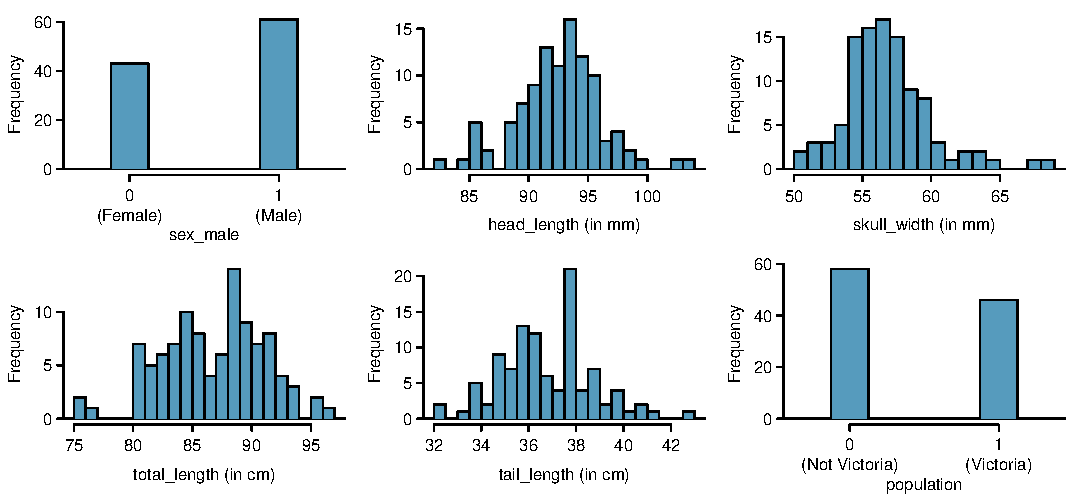
\includegraphics[width=\textwidth]{ch_regr_mult_and_log/figures/eoce/possumGLM/possumVars} 
\end{center}

\begin{center}\footnotesize
\begin{tabular}{r rrrr r rrrr}
& \multicolumn{4}{c}{\emph{Full Model}} &
& \multicolumn{4}{c}{\emph{Reduced Model}}  \\
  \cline{2-5}\cline{7-10}
\vspace{-3.1mm} \\
 & Estimate & SE & Z & Pr($>$$|$Z$|$) &
 & Estimate & SE & Z & Pr($>$$|$Z$|$) \\ 
  \hline
\vspace{-3.1mm} \\
  (Intercept) & 39.2349 & 11.5368 & 3.40 & 0.0007 &
  	& 33.5095 & 9.9053 & 3.38 & 0.0007 \\ 
  sex\_\hspace{0.3mm}male & -1.2376 & 0.6662 & -1.86 & 0.0632 &
  	& -1.4207 & 0.6457 & -2.20 & 0.0278 \\ 
  head\_\hspace{0.3mm}length & -0.1601 & 0.1386 & -1.16 & 0.2480 \\ 
  skull\_\hspace{0.3mm}width & -0.2012 & 0.1327 & -1.52 & 0.1294 &
  	& -0.2787 & 0.1226 & -2.27 & 0.0231\\ 
  total\_\hspace{0.3mm}length & 0.6488 & 0.1531 & 4.24 & 0.0000 &
  	& 0.5687 & 0.1322 & 4.30 & 0.0000\\ 
  tail\_\hspace{0.3mm}length & -1.8708 & 0.3741 & -5.00 & 0.0000 &
  	& -1.8057 & 0.3599 & -5.02 & 0.0000\\ 
   \hline
\end{tabular}
\end{center}

\begin{parts}
\item Examine each of the predictors. Are there any outliers that are likely to have a very large influence on the logistic regression model?
\item The summary table for the full model indicates that at least one variable should be eliminated when using the p-value approach for variable selection: \var{head\_\hspace{0.3mm}length}. The second component of the table summarizes the reduced model following variable selection. Explain why the remaining estimates change between the two models.
\end{parts}
}{}

\textB{\newpage}

% 14

\eoce{\qt{Challenger disaster, Part I} \label{ChallengerDisasterPartI} On January 28, 1986, a routine launch was anticipated for the Challenger space shuttle. Seventy-three seconds into the flight, disaster happened: the shuttle broke apart, killing all seven crew members on board. An investigation into the cause of the disaster focused on a critical seal called an O-ring, and it is believed that damage to these O-rings during a shuttle launch may be related to the ambient temperature during the launch. The table below summarizes observational data on O-rings for 23 shuttle missions, where the mission order is based on the temperature at the time of the launch. \emph{Temp} gives the temperature in Fahrenheit, \emph{Damaged} represents the number of damaged O-rings, and \emph{Undamaged} represents the number of O-rings that were not damaged.
\begin{center}\footnotesize
\begin{tabular}{l rrrrr rrrrr rrrrr rrrrr rrr}
\hline
\vspace{-3.1mm} \\
Shuttle Mission & 1 & 2 & 3 & 4 & 5 & 6 & 7 & 8 & 9 & 10 & 11 & 12 \\
\hline
\vspace{-3.1mm} \\
Temperature & 53 & 57 & 58 & 63 & 66 & 67 & 67 & 67 & 68 & 69 & 70 & 70  \\
Damaged & 5 & 1 & 1 & 1 & 0 & 0 & 0 & 0 & 0 & 0 & 1 & 0  \\
Undamaged & 1 & 5 & 5 & 5 & 6 & 6 & 6 & 6 & 6 & 6 & 5 & 6 \\
\hline
\\ 
\cline{1-12}
\vspace{-3.1mm} \\
Shuttle Mission & 13 & 14 & 15 & 16 & 17 & 18 & 19 & 20 & 21 & 22 & 23 \\
\cline{1-12}
\vspace{-3.1mm} \\
Temperature & 70 & 70 & 72 & 73 & 75 & 75 & 76 & 76 & 78 & 79 & 81 \\
Damaged & 1 & 0 & 0 & 0 & 0 & 1 & 0 & 0 & 0 & 0 & 0 \\
Undamaged & 5 & 6 & 6 & 6 & 6 & 5 & 6 & 6 & 6 & 6 & 6 \\
\cline{1-12}
\end{tabular}
\end{center}

\begin{parts}
\item Each column of the table above represents a different shuttle mission. Examine these data and describe what you observe with respect to the relationship between temperatures and damaged O-rings.
\item Failures have been coded as 1 for a damaged O-ring and 0 for an undamaged O-ring, and a logistic regression model was fit to these data. A summary of this model is given below. Describe the key components of this summary table in words.
\begin{center}
\begin{tabular}{rrrrr}
  \hline
 & Estimate & Std. Error & z value & Pr($>$$|$z$|$) \\ 
  \hline
(Intercept) & 11.6630 & 3.2963 & 3.54 & 0.0004 \\ 
Temperature & -0.2162 & 0.0532 & -4.07 & 0.0000 \\ 
   \hline
\end{tabular}
\end{center}
\item Write out the logistic model using the point estimates of the model parameters.
\item Based on the model, do you think concerns regarding O-rings are justified? Explain.
\end{parts}
}{}

% 15

\eoce{\qt{Possum classification, Part II} A logistic regression model was proposed for classifying common brushtail possums into their two regions in Exercise~\ref{possumClassification1}. Use the results of the summary table for the reduced model presented in Exercise~\ref{possumClassification1} for the questions below. The outcome variable took value 1 if the possum was from Victoria and 0 otherwise.
\begin{parts}
\item Write out the form of the model. Also identify which of the following variables are positively associated (when controlling for other variables) with a possum being from Victoria: \var{skull\_\hspace{0.3mm}width}, \var{total\_\hspace{0.3mm}length}, and \var{tail\_\hspace{0.3mm}length}.
\item Suppose we see a brushtail possum at a zoo in the US, and a sign says the possum had been captured in the wild in Australia, but it doesn't say which part of Australia. However, the sign does indicate that the possum is male, its skull is about 63 mm wide, its tail is 37 cm long, and its total length is 83 cm. What is the reduced model's computed probability that this possum is from Victoria? How confident are you in the model's accuracy of this probability calculation?
%logitp <- 33.5095 - 1.4207 - 0.2787*63 + 0.5687*83 - 1.8057*37; exp(logitp)/(1+exp(logitp))
\end{parts}
}{}

\textB{\newpage}

% 16

\eoce{\qt{Challenger disaster, Part II} Exercise~\ref{ChallengerDisasterPartI} introduced us to O-rings that were identified as a plausible explanation for the breakup of the Challenger space shuttle 73 seconds into takeoff in 1986. The investigation found that the ambient temperature at the time of the shuttle launch was closely related to the damage of O-rings, which are a critical component of the shuttle. See this earlier exercise if you would like to browse the original data.
\begin{center}
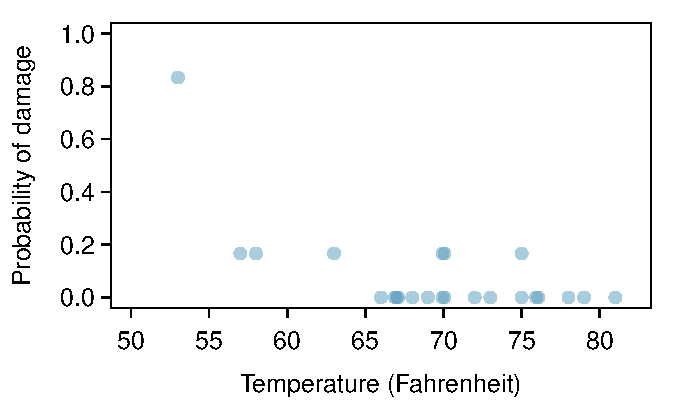
\includegraphics[width=0.6\textwidth]{ch_regr_mult_and_log/figures/eoce/challengerGLM/oringsData} 
\end{center}
\begin{parts}
\item The data provided in the previous exercise are shown in the plot. The logistic model fit to these data may be written as
\begin{align*}
\log\left( \frac{\hat{p}}{1 - \hat{p}} \right) = 11.6630 - 0.2162\times Temperature
\end{align*}
where $\hat{p}$ is the model-estimated probability that an O-ring will become damaged. Use the model to calculate the probability that an O-ring will become damaged at each of the following ambient temperatures: 51, 53, and 55 degrees Fahrenheit. The model-estimated probabilities for several additional ambient temperatures are provided below, where subscripts indicate the temperature:
\begin{align*}
&\hat{p}_{57} = 0.341
	&& \hat{p}_{59} = 0.251
	&& \hat{p}_{61} = 0.179
	&& \hat{p}_{63} = 0.124 \\
&\hat{p}_{65} = 0.084
	&& \hat{p}_{67} = 0.056
	&& \hat{p}_{69} = 0.037
	&& \hat{p}_{71} = 0.024
\end{align*}
\item Add the model-estimated probabilities from part~(a) on the plot, then connect these dots using a smooth curve to represent the model-estimated probabilities.
\item Describe any concerns you may have regarding applying logistic regression in this application, and note any assumptions that are required to accept the model's validity.
\end{parts}
}{}